\documentclass{beamer}
\usepackage[utf8]{inputenc}

\usetheme{Madrid}
\usecolortheme{default}
\usepackage{amsmath,amssymb,amsfonts,amsthm}
\usepackage{txfonts}
\usepackage{tkz-euclide}
\usepackage{listings}
\usepackage{adjustbox}
\usepackage{array}
\usepackage{tabularx}
\usepackage{gvv}
\usepackage{lmodern}
\usepackage{circuitikz}
\usepackage{tikz}
\usepackage{graphicx}
\usepackage{amsmath}

\setbeamertemplate{page number in head/foot}[totalframenumber]

\usepackage{tcolorbox}
\tcbuselibrary{minted,breakable,xparse,skins}



\definecolor{bg}{gray}{0.95}
\DeclareTCBListing{mintedbox}{O{}m!O{}}{%
  breakable=true,
  listing engine=minted,
  listing only,
  minted language=#2,
  minted style=default,
  minted options={%
    linenos,
    gobble=0,
    breaklines=true,
    breakafter=,,
    fontsize=\small,
    numbersep=8pt,
    #1},
  boxsep=0pt,
  left skip=0pt,
  right skip=0pt,
  left=25pt,
  right=0pt,
  top=3pt,
  bottom=3pt,
  arc=5pt,
  leftrule=0pt,
  rightrule=0pt,
  bottomrule=2pt,
  toprule=2pt,
  colback=bg,
  colframe=orange!70,
  enhanced,
  overlay={%
    \begin{tcbclipinterior}
    \fill[orange!20!white] (frame.south west) rectangle ([xshift=20pt]frame.north west);
    \end{tcbclipinterior}},
  #3,
}
\lstset{
    language=C,
    basicstyle=\ttfamily\small,
    keywordstyle=\color{blue},
    stringstyle=\color{orange},
    commentstyle=\color{green!60!black},
    numbers=left,
    numberstyle=\tiny\color{gray},
    breaklines=true,
    showstringspaces=false,
}


\title 
{4.12.28}



\author 
{Pratik R-AI25BTECH11023}



\begin{document}


\frame{\titlepage}
%------------------------------------
\begin{frame}{Question}
The value of the $\lambda$,  if the lines\\$(2x+3y+4)+\lambda(6x-y+12)=0$ are
\end{frame}

\begin{frame}{Table}
    \begin{tabular}[12pt]{ |c| c|}
    \hline
    \textbf{Points} & \textbf{Name}\\ 
    \hline
	\myvec{7\\10} & Point $\Vec{A}$ \\
    \hline 
	\myvec{-2\\5} & Point $\Vec{B}$\\
    \hline
	\myvec{3\\4} & Point $\Vec{C}$\\
    \hline
\end{tabular}
\end{frame}
\begin{frame}{Solution} 
Equation of line is given by
\begin{align}
    \myvec{2+6\lambda &3-\lambda} \vec{x} &=-4-12\lambda\\
    \implies n^\top x &= c;
\end{align}
where $\vec{n}^\top = \myvec{2+6\lambda &3-\lambda}$\\
and $c=-4-12\lambda$. \\
\end{frame}
\begin{frame}{Option 1}
If the line is parallel to Y axis
\begin{align}
\vec{n}^\top \vec{e_2} &=0 \\
3 -\lambda &= 0 \\
\lambda &= 3
\end{align}
\end{frame}

\begin{frame}{Option 2}
If the line is perpendicular to $7x+y-4=0$, that is, $\vec{n_1}^\top =\myvec{7&1}$
\begin{align}
    \vec{n_1}^\top \vec{n} &= 0 \\
    41\lambda &= -17 \\
    \lambda &= \frac{-17}{41}
\end{align}
\end{frame}

\begin{frame}{Option 3}
If the line passes through $P(1,2)$
\begin{align}
  \vec{n}^\top \vec{P} &= c \\
  16\lambda &= -12 \\
  \lambda &= \frac{-3}{4}
\end{align}
\end{frame}
\begin{frame}{Option 4}
If the line is parallel to X axis
\begin{align}
\vec{n}^\top \vec{e_1} &=0 \\
2+6\lambda &= 0 \\
\lambda &= \frac{-1}{3}
\end{align}
\end{frame}
\begin{frame}{plot}
\centering
    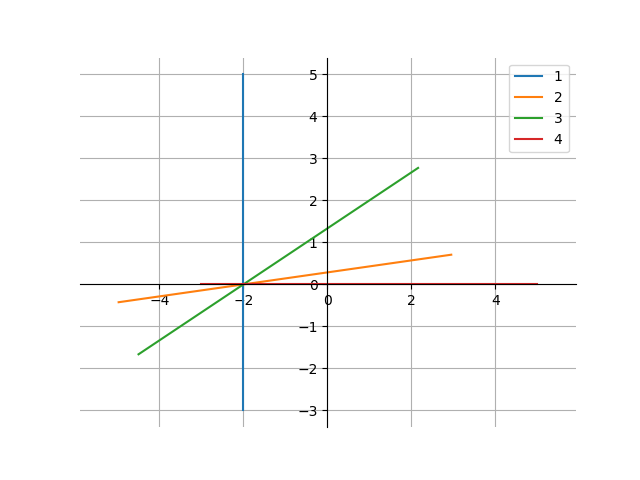
\includegraphics[width=\columnwidth, height=0.8\textheight, keepaspectratio]{../figs/fig.png}     
\end{frame}


\end{document}